%!TEX program = xelatex
\documentclass[dvipsnames, svgnames,a4paper,11pt]{article}
% ----------------------------------------------------
%   吉林大学通信工程学院信号与系统实验报告
%   原作者:Huanyu Shi,2019级
%     知乎:https://www.zhihu.com/people/za-ran-zhu-fu-liu-xing
%     Github:https://github.com/huanyushi/SYSU-SPA-Labreport-Template
%   在原基础上魔改了一些,更加贴近吉林大学实验格式。
% ----------------------------------------------------

% ----------------------------------------------------- 
%	加边框的命令
%	参考:https://tex.stackexchange.com/questions/531559/how-to-add-the-page-border-for-first-two-pages-in-latex
\usepackage{tikz}
\usetikzlibrary{calc}
\usepackage{eso-pic}
\AddToShipoutPictureBG{%
\begin{tikzpicture}[overlay,remember picture]
\draw[line width=0.6pt] % 边框粗细
    ($ (current page.north west) + (0.6cm,-0.6cm) $)
    rectangle
    ($ (current page.south east) + (-0.6cm,0.6cm) $); % 边框位置
\end{tikzpicture}}


\usepackage{xcolor}
\definecolor{c1}{HTML}{2752C9} % 目录颜色
\definecolor{c2}{RGB}{190,20,83} % 引用颜色

\usepackage{ctex}
\usepackage[top=28mm,bottom=28mm,left=15mm,right=15mm]{geometry}
\usepackage{hyperref} 
\hypersetup{
	colorlinks,
	linktoc = section, % 超链接位置,选项有section, page, all
	linkcolor = c1, % linkcolor 目录颜色
	citecolor = c1  % citecolor 引用颜色
}
\usepackage{amsmath,enumerate,multirow,float}
\usepackage{tabularx}
\usepackage{tabu}
\usepackage{subfig}
\usepackage{fancyhdr}
\usepackage{graphicx}
\usepackage{wrapfig}  
\usepackage{physics}
\usepackage{appendix}
\usepackage{amsfonts}

%
\usepackage{tcolorbox}
\tcbuselibrary{skins,breakable}
\newtcolorbox{tbox}[2][]{
    colframe=black!70!,
    breakable,
    enhanced,
	boxrule =0.5pt,
    title = {#2},
    fonttitle = \large\kaishu\bfseries,
	drop fuzzy shadow,
    #1
}
\newtcolorbox[auto counter,number within=section]{question}[1][]{
  top=2pt,bottom=2pt,arc=1mm,
  boxrule=0.5pt,
%   frame hidden,
  breakable,
  enhanced, %跨页后不会显示下边框
  coltitle=c1!80!gray,
  colframe=c1,
  colback=c1!3!white,
  drop fuzzy shadow,
  title={思考题~\thetcbcounter:\quad},
  fonttitle=\bfseries,
  attach title to upper,
  #1
}

% ---------------------------------------------------------------------
%	利用cleveref改变引用格式,\cref是引用命令
\usepackage{cleveref}
\crefformat{figure}{#2{\textcolor{c2}{图 #1}}#3} % 图片的引用格式
\crefformat{equation}{#2{(\textcolor{c2}{#1})}#3} % 公式的引用格式
\crefformat{table}{#2{\textcolor{c2}{表 #1}}#3} % 表格的引用格式


% ---------------------------------------------------------------------
%	页眉页脚设置
\fancypagestyle{plain}{\pagestyle{fancy}}
\pagestyle{fancy}
\lhead{\kaishu 吉林大学通信工程学院} % 左边页眉,学院 + 课程
\rhead{\kaishu 信号与系统实验报告} % 右边页眉,实验报告标题
\cfoot{\thepage} % 页脚,中间添加页码


% ---------------------------------------------------------------------
%	对目录、章节标题的设置
\renewcommand{\contentsname}{\centerline{\huge 目录}}
\usepackage{titlesec}
\usepackage{titletoc}
% \titleformat{章节}[形状]{格式}{标题序号}{序号与标题间距}{标题前命令}[标题后命令]
\titleformat{\section}{\centering\LARGE\songti}{}{1em}{}

% ---------------------------------------------------------------------
%   listing代码环境设置
\usepackage{listings}
\lstloadlanguages{python}
\lstdefinestyle{pythonstyle}{
backgroundcolor=\color{gray!5},
language=python,
frameround=tftt,
frame=shadowbox, 
keepspaces=true,
breaklines,
columns=spaceflexible,                   
basicstyle=\ttfamily\small, % 基本文本设置,字体为teletype,大小为scriptsize
keywordstyle=[1]\color{c1}\bfseries, 
keywordstyle=[2]\color{Red!70!black},   
stringstyle=\color{Purple},       
showstringspaces=false,
commentstyle=\ttfamily\scriptsize\color{green!40!black},%注释文本设置,字体为sf,大小为smaller
tabsize=2,
morekeywords={as},
morekeywords=[2]{np, plt, sp},
numbers=left, % 代码行数
numberstyle=\it\tiny\color{gray}, % 代码行数的数字字体设置
stepnumber=1,
rulesepcolor=\color{gray!30!white}
}




% ---------------------------------------------------------------------
%	其他设置
\def\degree{${}^{\circ}$} % 角度
\graphicspath{{./images/}} % 插入图片的相对路径
\allowdisplaybreaks[4]  %允许公式跨页


%---------------------------------------------------------------------------%
%->> User defined commands
%---------------------------------------------------------------------------%
\RequirePackage{mathrsfs}% script style math symbols % 导入模板的相关设置
\usepackage{lipsum}


%---------------------------------------------------------------------
%	正文
%---------------------------------------------------------------------

\begin{document}

\begin{table}
  \raggedleft
	\renewcommand\arraystretch{1.7}
	\begin{tabular}{|c|p{4em}|}
	\hline
	成绩 &  \\
	\hline
	教师签字 &   \\
	\hline
	\end{tabular}
\end{table}

\begin{center}
	{\kaishu \LARGE   \quad  \quad 通  \quad 信  \quad 工  \quad 程  \quad 学  \quad 院 }
  \newline
  \newline
  \newline
  \newline
  \newline
  {\kaishu \Huge 实 \quad  \quad  \quad 验  \quad  \quad  \quad 报 \quad  \quad  \quad 告}
  \newline
  \newline
  \newline
  \newline
  \newline
  {\songti \Huge  ( \quad  信  \quad 号  \quad 与  \quad 系  \quad 统 \quad)}
  \newline
  \newline
  \newline
  \newline
  \newline
  {\songti  \LARGE 实验题目:信号的采样与恢复  \quad  \quad \quad}
\end{center}



\begin{table}[b]
	\renewcommand\arraystretch{1.7}
	\begin{tabularx}{\textwidth}{|X|X|X|X|}
	\hline
	专业:& 通信工程 &年级:& 2022级\\
	\hline
	姓名:& 苏睿杰  & 学号:& 20220826\\
	\hline
	实验时间:& 2023年11月17日 & 班级:& 42 \\
	\hline
	\end{tabularx}
\end{table}


%\clearpage
%\tableofcontents

\clearpage
\setcounter{section}{0}
\section{实验二十一 \quad 信号的采样与恢复}
\subsection*{一、实验目的}
\begin{enumerate}
  \item 掌握低通滤波电路的通频带的测量方法。
  \item 了解电信号的采样方法与过程及信号的恢复。
  \item 验证采样定理。
\end{enumerate}

\subsection*{二、实验仪器}
\begin{enumerate}
  \item 信号与系统实验箱一台
  \item 数宇示波器一台
  \item 数宇信号发生器
  \item 交流毫伏表
\end{enumerate}

\subsection*{三、实验原理}

\begin{enumerate}
  \item 离散时间信号可以从离散信号源获得,也可以从连续时间信号采样而得。采样信号 $f_s(t)$ 可以看成连续信号 $f(t)$ 和一组开关函数 $s(t)$ 的乘积。$s(t)$ 是一组周期性窄脉冲。对采样信号进行傅立叶分析可知,采样信号的频率包括了原连续信号以及无限个经过平移的原信号频率。平移的频率等于采样频率 $f_s$ 及其谐波频率 $2f_s$、$3f_s$...。
  \item 抽样信号在一定条件下可以恢复原来的信号,只要用一截上频率等于原信号频谱中最高频率 $f_n$ 的低通滤波器,滤除高频分量,经滤波后得到的信号包含了原信号频谱的全部内容,即低通滤波器的输出可以得到恢复后的信号。
  \item 原信号得以恢复的条件是 $f_s \ge 2B$,其中 $f_s$ 为采样频率,$B$ 为原信号占有的频带宽度。$f_{min}=2B$ 为最低采样频率。当 $f_s < 2B$ 时,采样信号的频谱会发生混叠;所以无法用低通滤波器获得原信号频谱的全部内容。在实际使用时,仅包含有限频率的信号是极少的,因此即使 $f_s=2B$,恢复后的信号失真还是难免的。
  
  实验中选用 $f_s<2B$,$f_s=2B$,$f_s>2B$ 三种抽样频率对连续信号进行采样,以验证采样定理。要使信号采样后能不失真的还原,采样频率 $f_s$ 必领远大于信号频率中最高频率的两倍。采样频率一般为信号频率四倍以上。
  \item 为了实现对连续信号的采样和对采样信号的复原,可用实验原理框图1所示。除选用足够高的采样频率外,常采用前置低通滤波器来防止信号频谱过宽而造成采样后信号频谱的混叠。
  \begin{figure}[htbp]
    \centering
    \subfloat[]{
      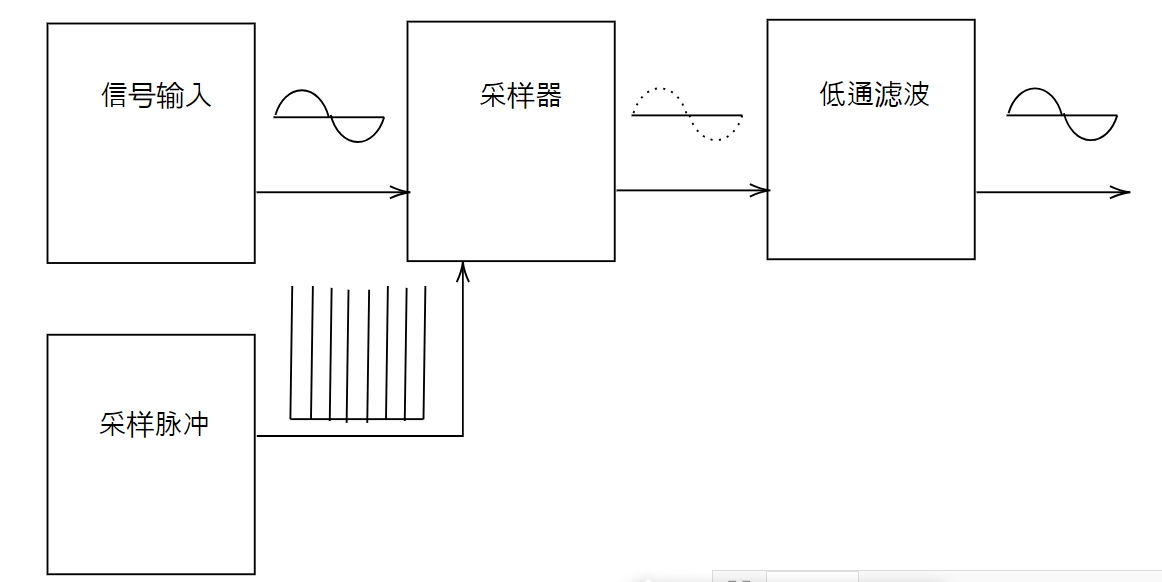
\includegraphics[width=0.7\textwidth]{1.png}
    }
    \caption{信号的采样与恢复原理框图}
  \end{figure}
\end{enumerate}

\subsection*{四、实验内容与步骤}
\begin{enumerate}
  \item 输入信号为 $5KHz$ 的方波信号,$V_{p-p} = 2V$,观察抽样后离散方波信号的波形并用通过信号系统实验箱的低通滤波电路观察恢复后的信号波形。
  \item 测出信号系统实验箱上的低通滤波电路的通频带见图2,在不失真的条件下选择合适的输入信号的频率,并且选择合适的采样脉冲的频率进行抽样,再送到下述滤波电路中进行恢复记录并观察波形。
  \begin{figure}[htbp]
    \centering
    \begin{minipage}[t]{0.48\textwidth}
    \centering
    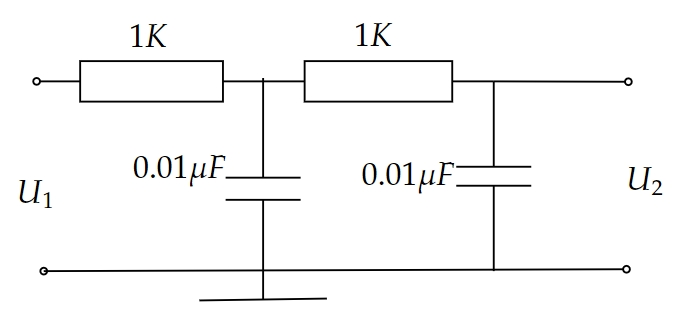
\includegraphics[width=6cm]{2-a.png}
    \caption{无源低通滤波器}
    \end{minipage}
    \begin{minipage}[t]{0.48\textwidth}
    \centering
    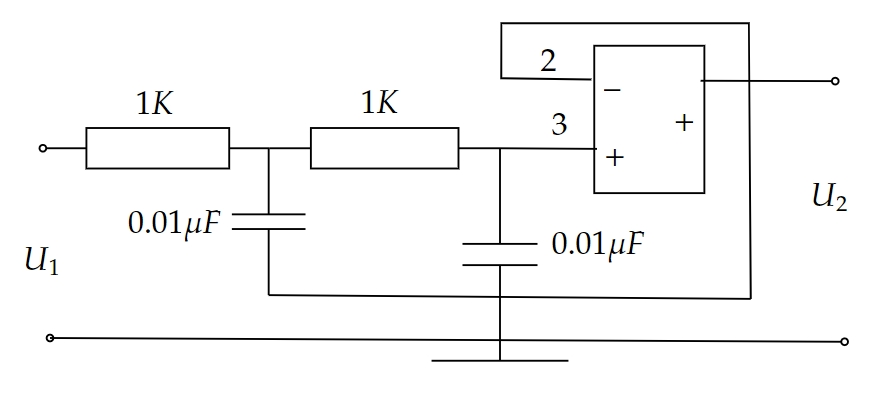
\includegraphics[width=9cm]{2-b.png}
    \caption{有源低通滤波器}
    \end{minipage}
  \end{figure}
\end{enumerate}

\newpage
\subsection*{五、数据记录与处理}
  \begin{enumerate}
    \item 输入信号为频率1kHz,峰峰值为$2V_{pp}$的方波。采样信号为频率可调的周期矩形脉冲。
      \begin{figure}[htbp]
        \centering
        \subfloat[]{
          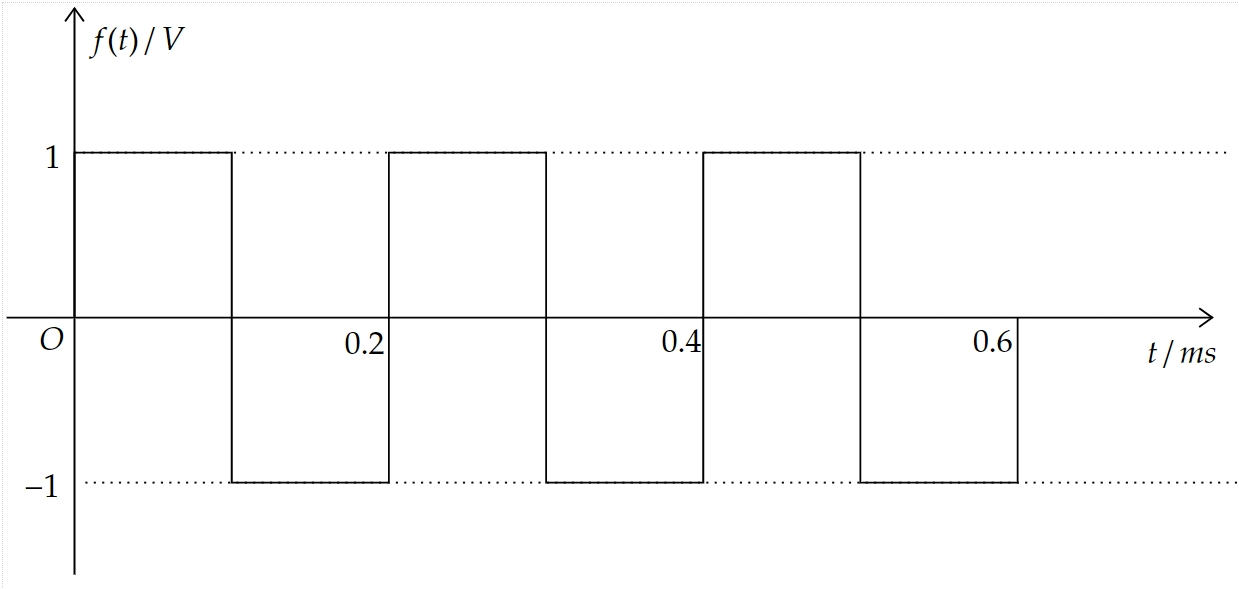
\includegraphics[width=0.5\textwidth]{3.png}
        }
        \subfloat[]{
          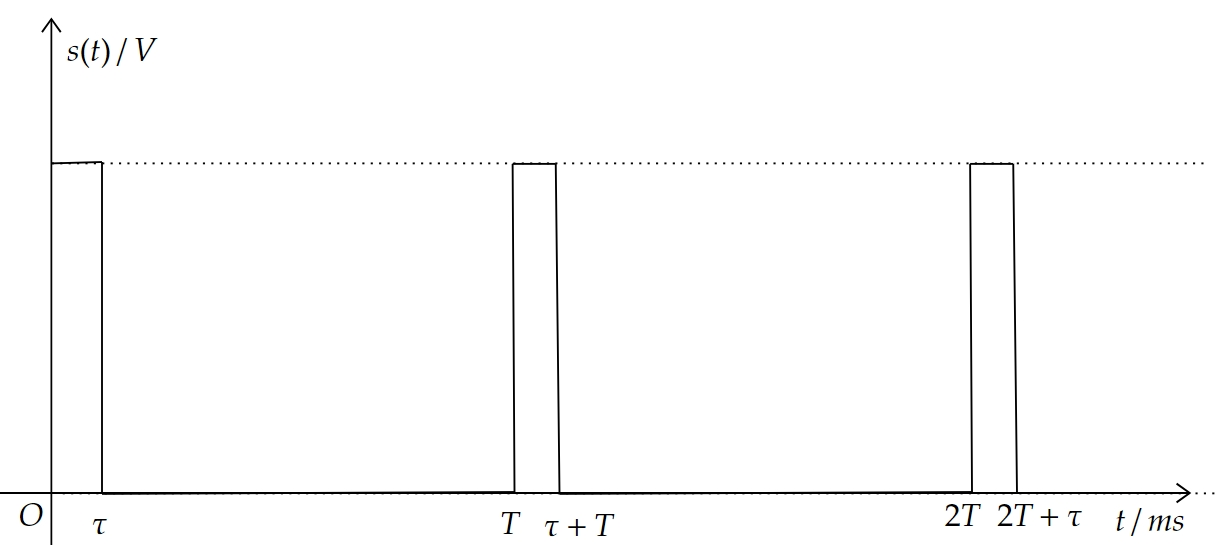
\includegraphics[width=0.5\textwidth]{6.png}
        }
        \caption{输入方波波形以及采样信号,带宽 B = 9kHz}
      \end{figure}
      \begin{figure}[htbp]
        \centering
        \subfloat[]{
          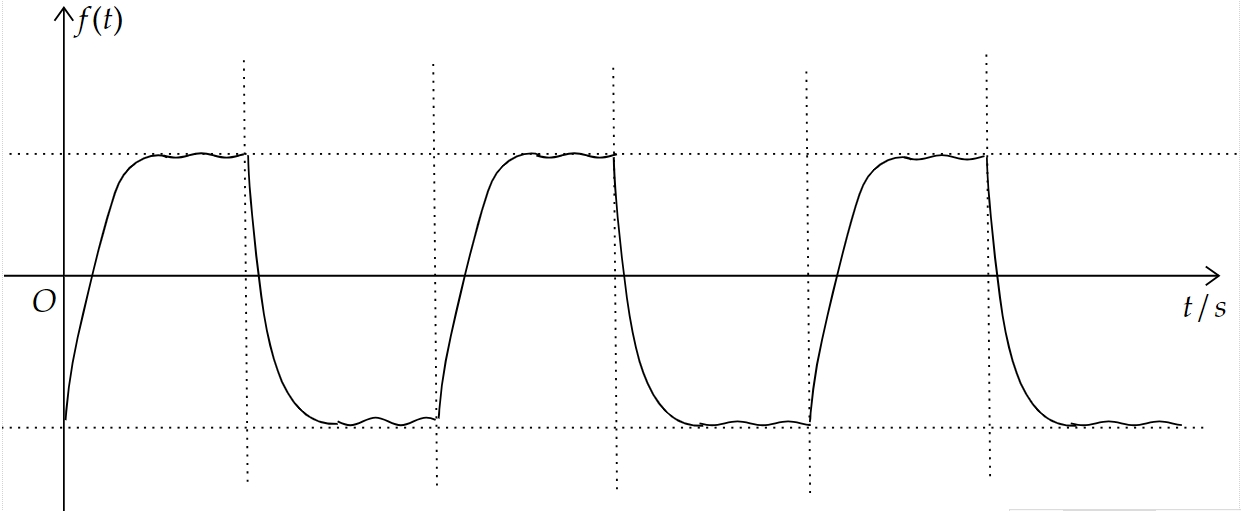
\includegraphics[width=0.5\textwidth]{3-1.png}
        }
        \subfloat[]{
          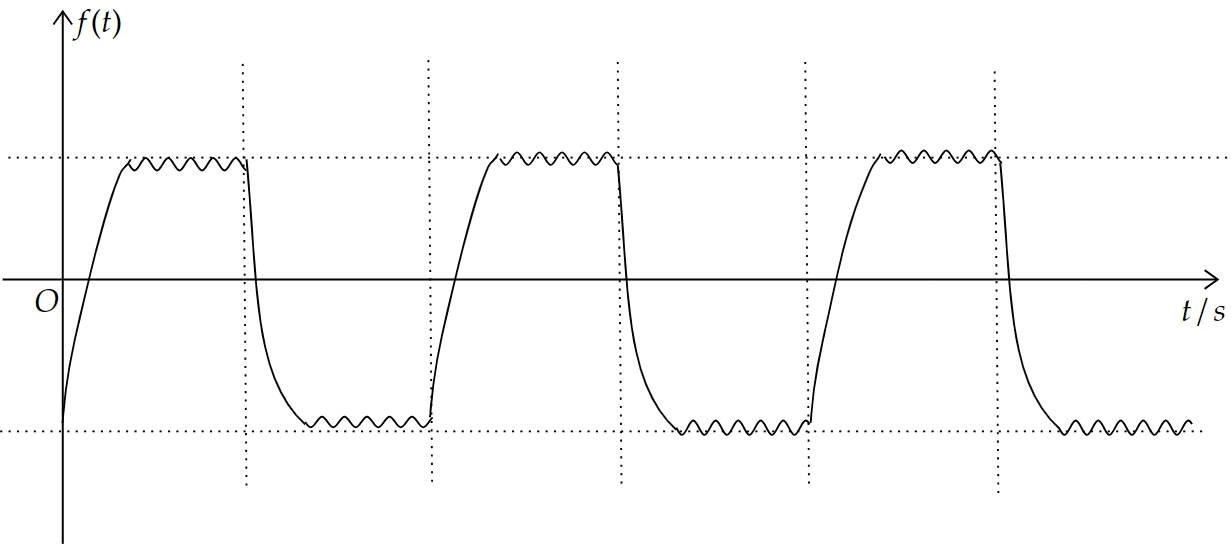
\includegraphics[width=0.5\textwidth]{3-2.png}
        }

        \subfloat[]{
          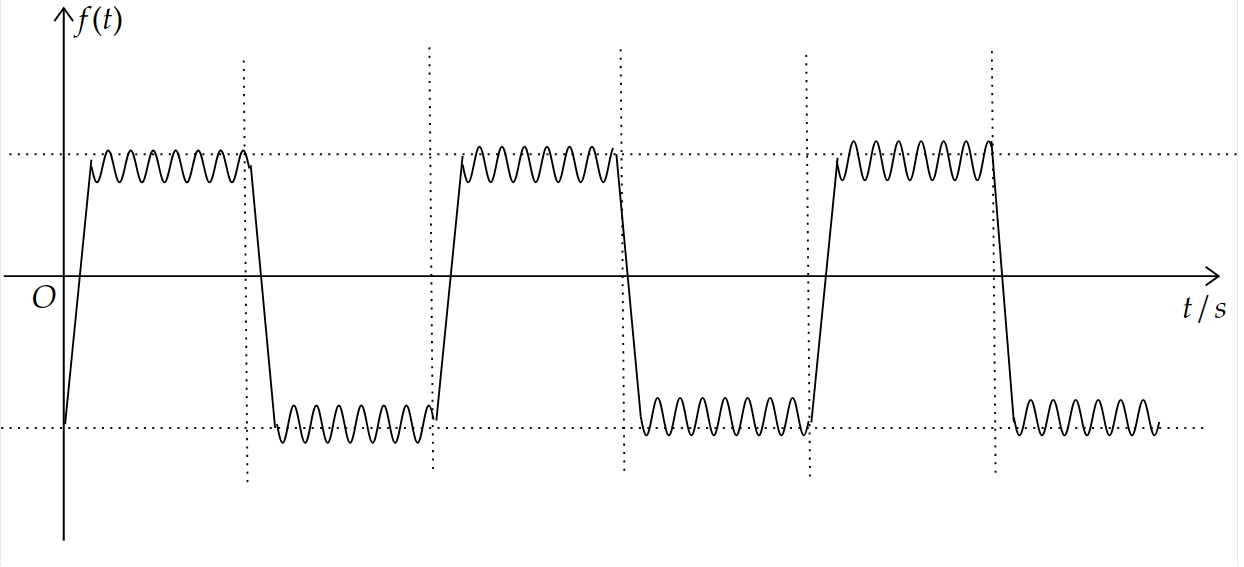
\includegraphics[width=0.5\textwidth]{3-3.png}
        }
        \caption{恢复后的方波波形}
      \end{figure}
      
      \begin{enumerate}
        \item 选取抽样频率 $fs = 30kHz > 2B$,得到恢复后的信号如图 5.a,其中恢复后的 $V_{pp} = 5.36V,f = 999.5Hz$。
        \item 选取抽样频率 $fs = 18kHz = 2B$,得到恢复后的信号如图 5.b,其中恢复后的 $V_{pp} = 5.68V,f = 997.5Hz$。
        \item 选取抽样频率 $fs = 10kHz < 2B$,得到恢复后的信号如图 5.c,其中恢复后的 $V_{pp} = 7.04,f = 992.1Hz$。
      \end{enumerate}


    \newpage
    \item 输入信号为频率 1kHz,峰峰值为 $2V_{pp}$ 的三角波。采样信号为频率可调的周期矩形脉冲。
      \begin{figure}[htbp]
        \centering
        \subfloat[]{
          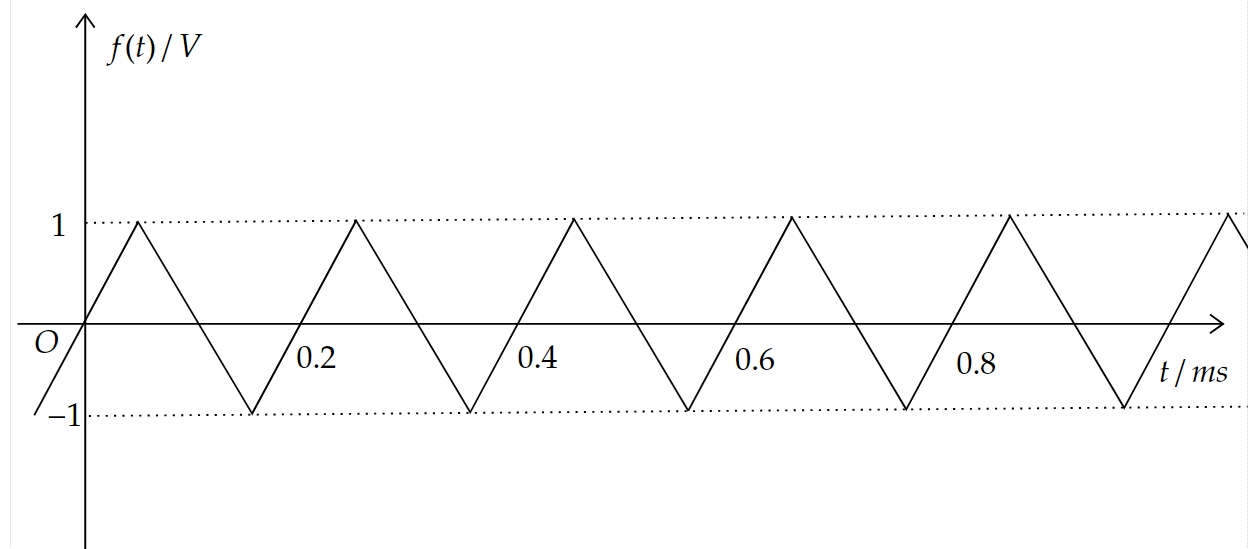
\includegraphics[width=0.5\textwidth]{4.png}
        }
        \subfloat[]{
          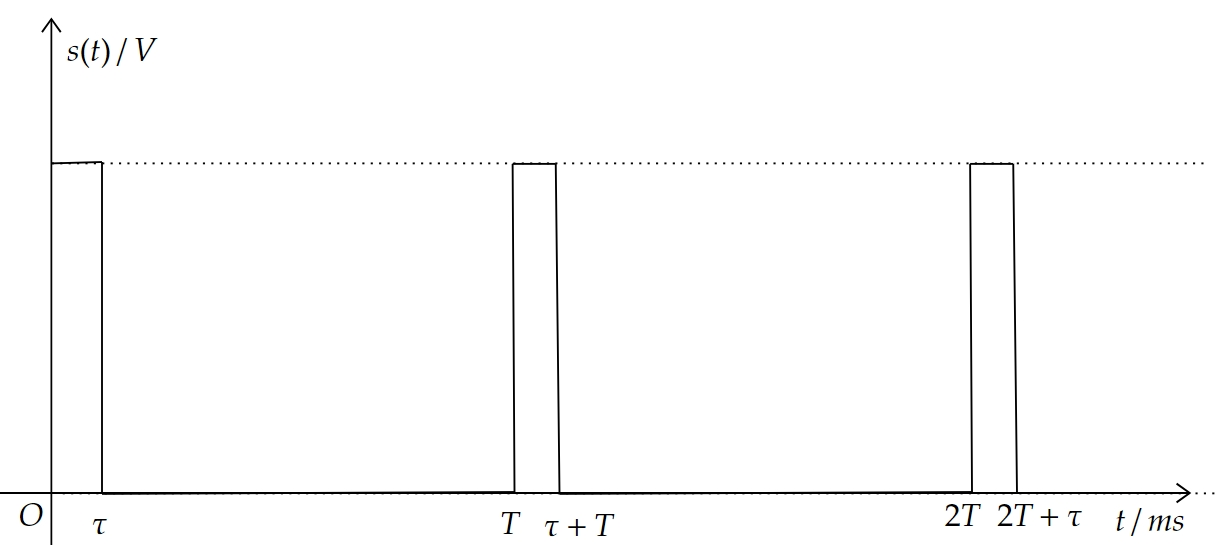
\includegraphics[width=0.5\textwidth]{6.png}
        }
        \caption{输入三角波波形以及采样信号,带宽 B = 3kHz}
      \end{figure}
      \begin{figure}[htbp]
        \centering
        \subfloat[]{
          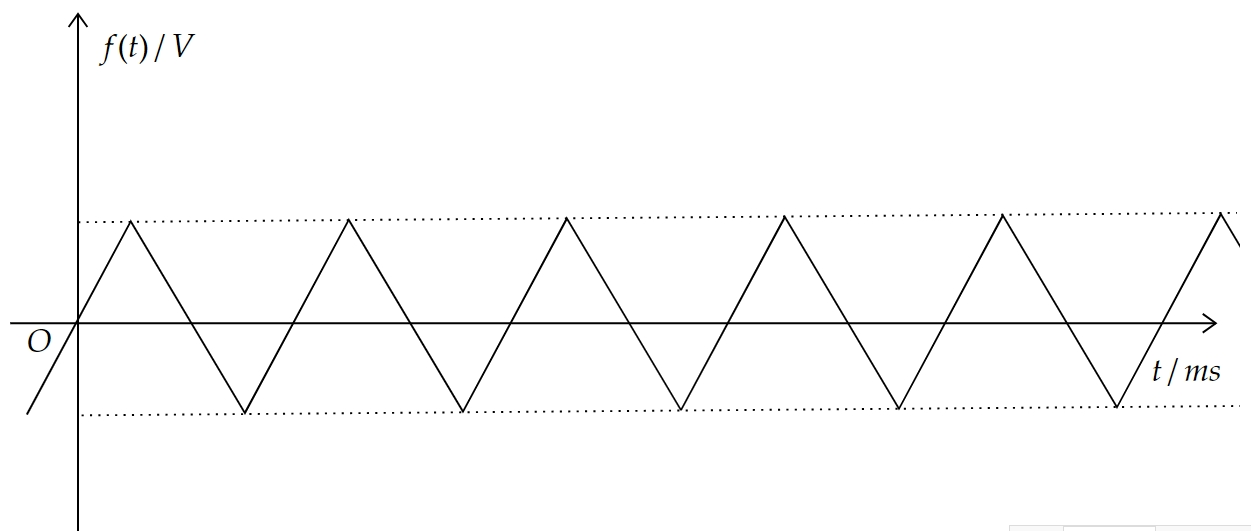
\includegraphics[width=0.5\textwidth]{4-1.png}
        }
        \subfloat[]{
          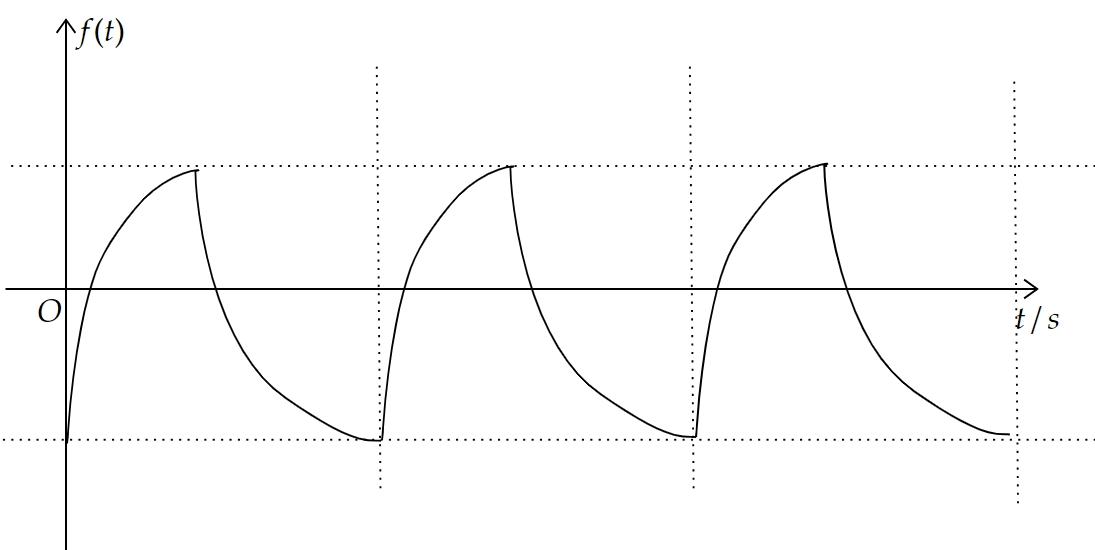
\includegraphics[width=0.5\textwidth]{4-2.png}
        }

        \subfloat[]{
          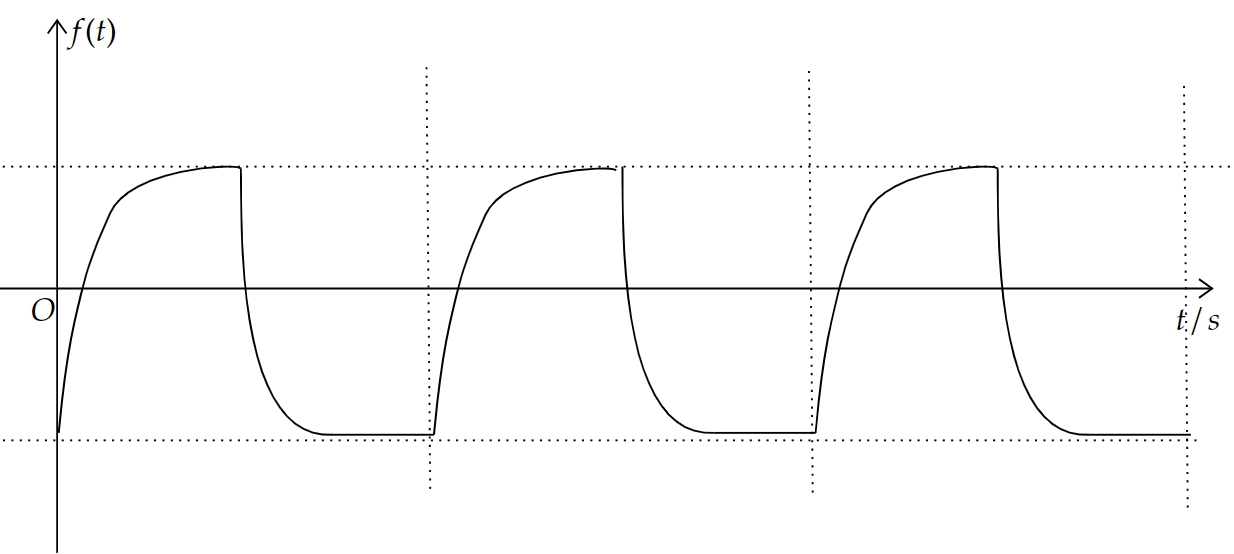
\includegraphics[width=0.5\textwidth]{4-3.png}
        }
        \caption{恢复后的三角波波形}
      \end{figure}

      \begin{enumerate}
        \item 选取抽样频率 $fs = 25kHz > 2B$,得到恢复后的信号如图 7.a,其中恢复后的 $V_{pp} = 2.4V,f = 25.1kHz$。
        \item 选取抽样频率 $fs = 6kHz = 2B$,得到恢复后的信号如图 7.b,其中恢复后的 $V_{pp} = 8.48V,f = 6.081kHz$。
        \item 选取抽样频率 $fs = 4kHz < 2B$,得到恢复后的信号如图 7.c,其中恢复后的 $V_{pp} = 10.2V,f = 4.029kHz$。
      \end{enumerate}
    
    \newpage
    \item 输入信号为频率 $1kHz$,峰峰值为 $2V_{pp}$ 的锯齿波。采样信号为频率可调的周期矩形脉冲。
      \begin{figure}[htbp]
        \centering
        \subfloat[]{
          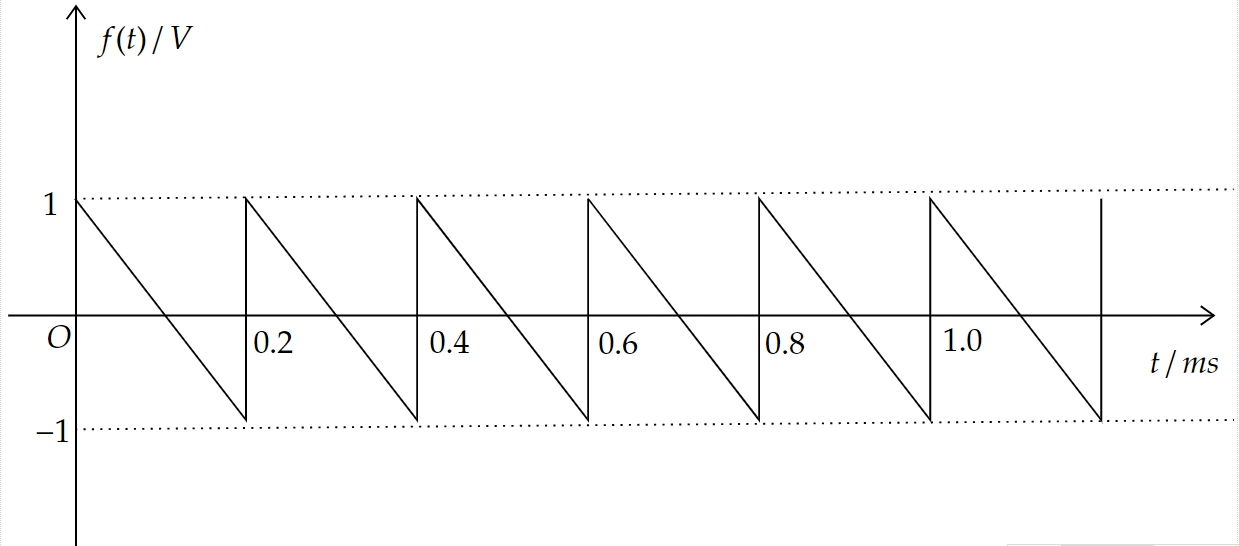
\includegraphics[width=0.5\textwidth]{5.png}
        }
        \subfloat[]{
          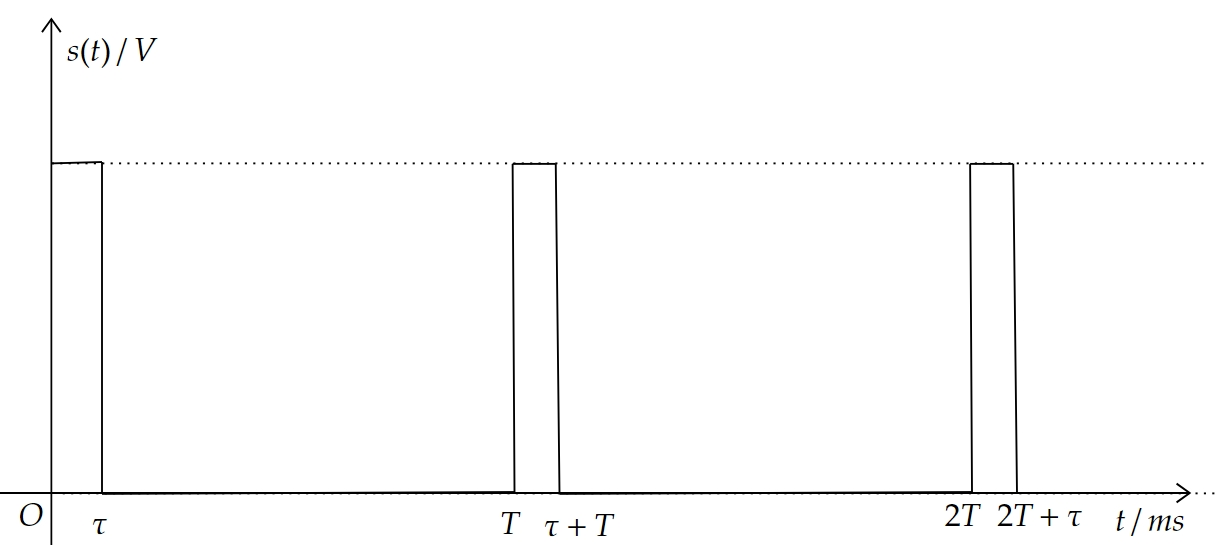
\includegraphics[width=0.5\textwidth]{6.png}
        }
        \caption{输入锯齿波波形以及采样信号,带宽 B = 10kHz}
      \end{figure}
      \begin{figure}[htbp]
        \centering
        \subfloat[]{
          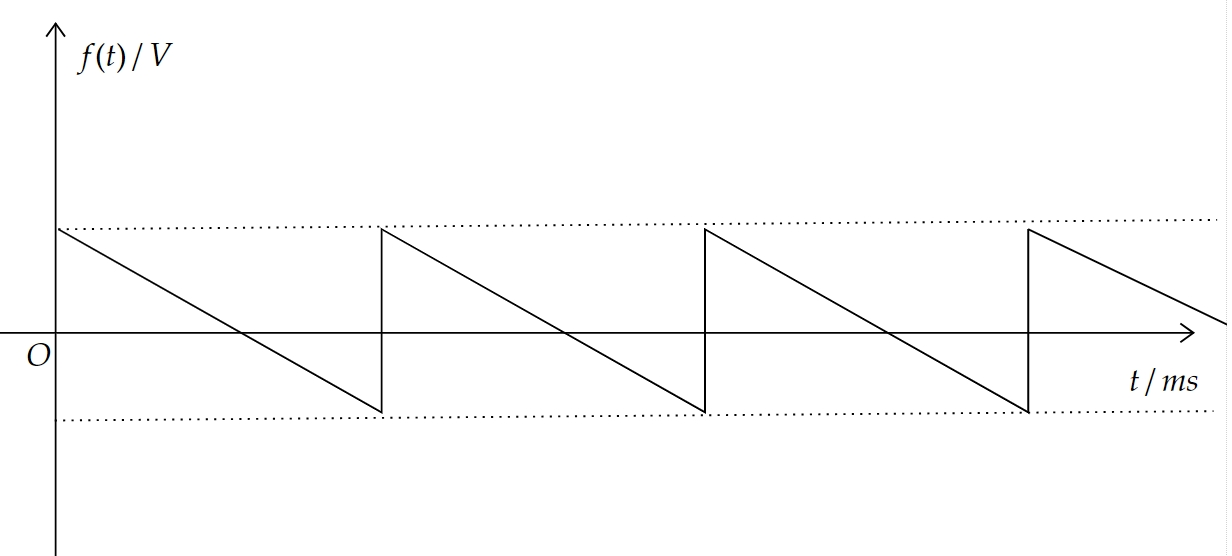
\includegraphics[width=0.5\textwidth]{5-1.png}
        }
        \subfloat[]{
          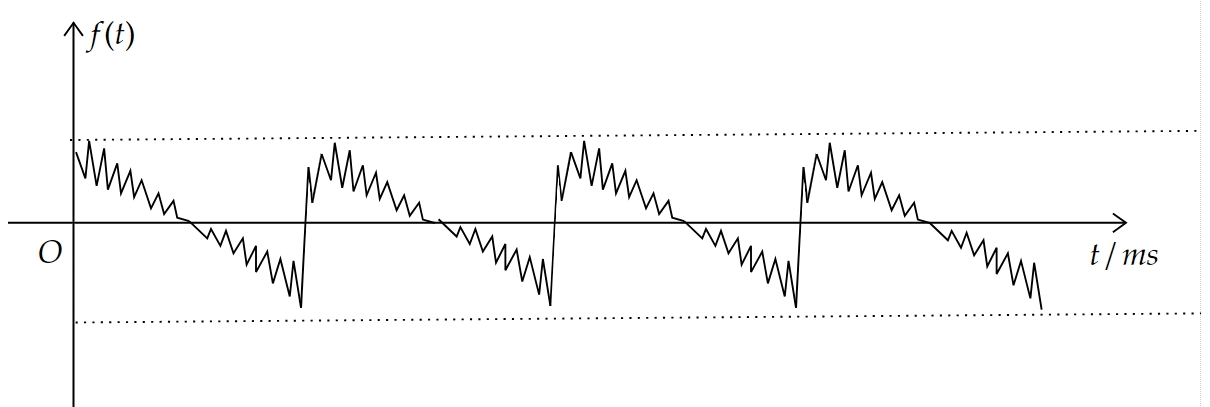
\includegraphics[width=0.5\textwidth]{5-2.png}
        }

        \subfloat[]{
          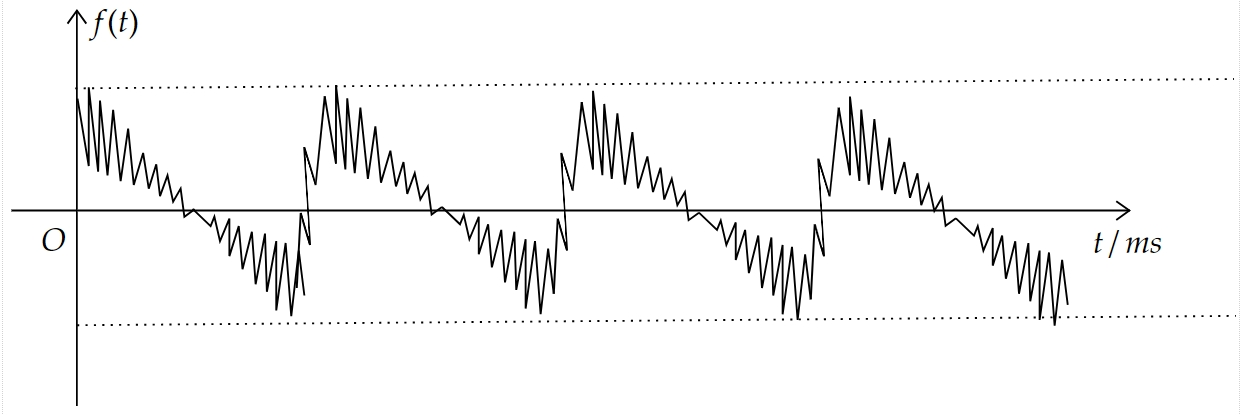
\includegraphics[width=0.5\textwidth]{5-3.png}
        }
        \caption{恢复后的锯齿波波形}
      \end{figure}

      \begin{enumerate}
        \item 选取抽样频率 $fs = 130kHz > 2B$,得到恢复后的信号如图 9.a,其中恢复后的 $V_{pp} = 0.92V,f = 1.004kHz$。
        \item 选取抽样频率 $fs = 20kHz = 2B$,得到恢复后的信号如图 9.b,其中恢复后的 $V_{pp} = 1.14V,f = 990.2Hz$。
        \item 选取抽样频率 $fs = 4kHz < 2B$,得到恢复后的信号如图 9.c,其中恢复后的 $V_{pp} = 1.66V,f = 1.007kHz$。
      \end{enumerate}

  \end{enumerate}

\newpage
\subsection*{六、实验误差分析}
\begin{enumerate}
  \item 在上述实验中,即使取 $fs > 2B$,我们还是发现恢复后的信号与输入信号有一定差别,个别恢复信号的峰峰值和频率与输入信号差别较大。这或许是因为采样频率还是不够大,并没有达到 \textbf{远大于} 最高频率的两倍,依然造成部分采样信号的频谱混叠。
\end{enumerate}
\subsection*{七、实验总结与思考}
\begin{enumerate}
  \item 当抽样频率 $f_s < 2B$ 时,此时复原后的函数失真较为严重,所得图像与 $f(t)$ 之间的误差较大。
  \item 当抽样频率 $f_s = 2B$ 时,此时复原后的函数有一定失真,但比 $f_s < 2B$ 时要好很多,所得图像已经较为接近输入信号。
  \item 当抽样频率 $f_s > 2B$ 时,此时复原后的函数几乎没有失真,所等图像与 $f(t)$ 最为接近,复原程度最好,最接近输入信号。从波形上已经非常接近输出信号,但是峰峰值数据以及频率依然和输入信号有一定差别。
\end{enumerate}

\end{document}